\frame{
\frametitle{Tree Decomposition}
    \begin{columns}
\column{0.4\textwidth}
\begin{wideitemize}
    \item Breaks down a rooted tree into smaller subparts to more efficiently solve subproblems
    \item Heavy-Light Decomposition 
    \begin{itemize}
        \item Separates edges into heavy ($\geq 1/2$ subtree size) and light ($< 1/2$ subtree size).
        \item Every path from root to leaf contains $\leq log_2(n)$ light edges.
    \end{itemize}
\end{wideitemize}
\column{0.6\textwidth}
    \centering
    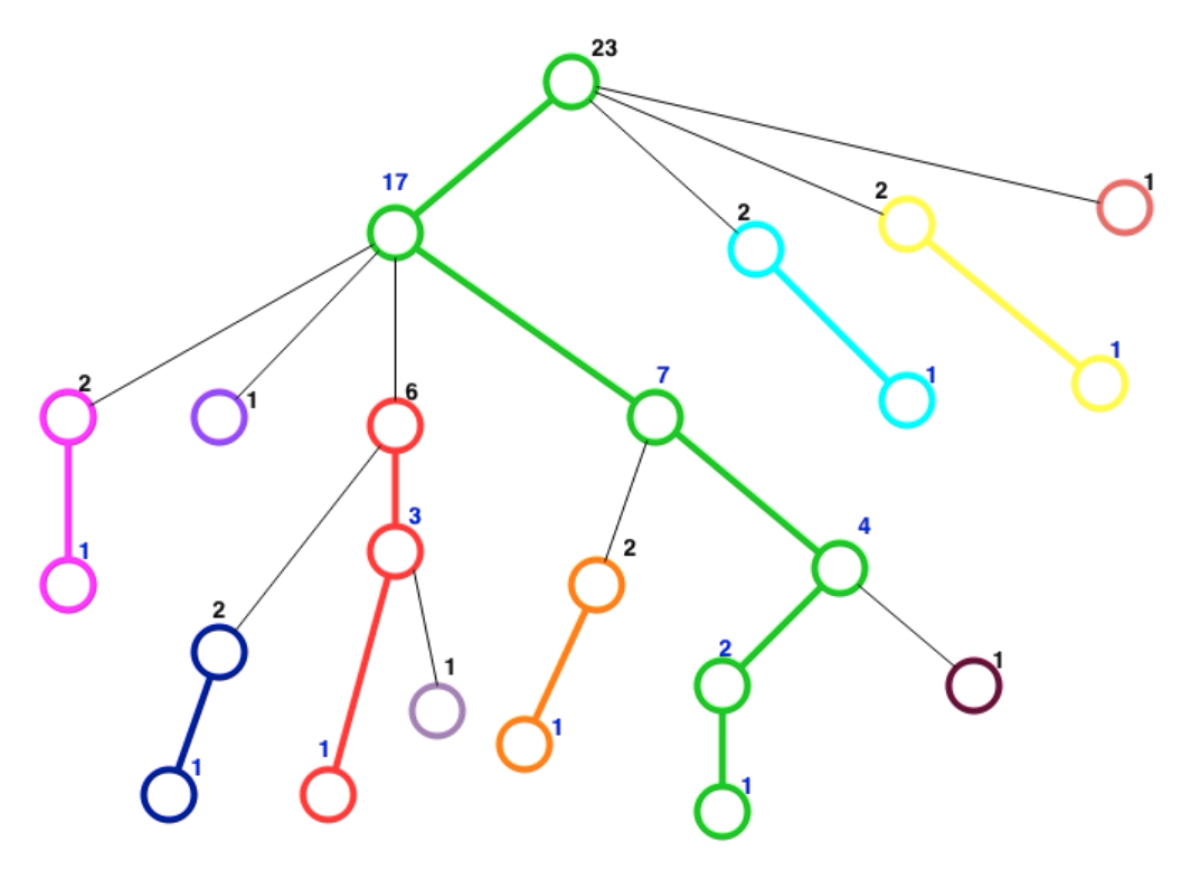
\includegraphics[scale=0.2]{slides/tree-decomp/heavy-light-decomposition-hld-0-1636267006.png}
  {\tiny \texttt{https://www.naukri.com/code360/library/heavy-light-decomposition-hld}}
    
\end{columns}
    
}
